%% ---------------------------------------------------------------------------
%% intro.tex
%%
%% Introduction
%%
%% ---------------------------------------------------------------------------

\chapter{Introducción}
\label{chp:intro}

\section{Contexto: Situación actual en Costa Rica}
Es bastante claro que, en todos los países, donde Costa Rica no es la excepción, existen personas que por razones de 
enfermedad, accidentes, vejez u otras situaciones, son declaradas con algún tipo de discapacidad y que de
manera parcial o total pierden la movilidad en su cuerpo. 

A manera de ejemplo y basados en el Vigésimo Segundo Informe Estado de la Nación en Desarrollo Humano Sostenible de 
Costa Rica \cite{estadonacion1}, en el capítulo 5 referente al Fortalecimiento de la Democracia se expresa lo siguiente: 

\begin{center}
“\textit{De acuerdo con el censo de 2011, en Costa Rica viven 452.849 personas con algún tipo de discapacidad, lo que
representa alrededor de un 10\% de la población total.}”

\end{center}
Esto hace pensar que una cantidad importante de personas en Costa Rica, y de hecho en todos los países del mundo, 
sufren de alguna discapacidad y basado en esto se pueden proponer soluciones a este problema que les garantice 
una mejor calidad de vida. 



Una de las principales prioridades de los profesionales, en este caso, la ingeniería, es buscar el bienestar de los
demás y lograr una vida digna para ellos, es por esto que el problema que afronta este proyecto es la dificultad de
ejecución de actividades cotidianas por parte de personas con algún tipo de discapacidad, y en este caso se enfoca
en la tarea de alcanzar objetos que se encuentran en su entorno. 

Aunque este trabajo puede ser ejecutado por personas capacitadas en esta área, esta tarea también puede ser ejecutada
por robots humanoides, capaces de cumplir con labores varias, y reubicar a este personal en actividades que requieran
habilidades más complejas para mejorar la atención a los pacientes. Por esta razón se propone implementar un sistema 
para la asistencia de pacientes mediante el robot Pepper.



La posibilidad de implementar un robot humanoide que pueda asistir al paciente facilita el cuidado que requieren
estas personas. Debido a que el proyecto se hará utilizando el robot humanoide Pepper, no existen opciones de 
selección de hardware, sino más bien, utilizando todo el potencial de este robot utilizar todas las herramientas
de software para ejecutar este proyecto de la mejor manera.  Los principales sistemas que posee este robot son
sensores como una unidad inercial, láseres, sensores infrarrojos, sensores ultrasónicos, codificadores rotativos 
magnéticos y sensores táctiles y de contacto; los sistemas de interacción contemplan altavoces, micrófonos, cámaras 2D,
sensor 3D (dispositivo tipo Kinect), LEDs, además los sistemas de movimiento y traslación contempla varios motores.\\
A continuación, se muestra en la Figura \ref{fig:RobotPepper} una fotografía del robot Pepper donde se pueden observar 
algunos de los módulos mencionados anteriormente. 
\vspace{0.2cm}


\begin{figure}[H]
	\centering
	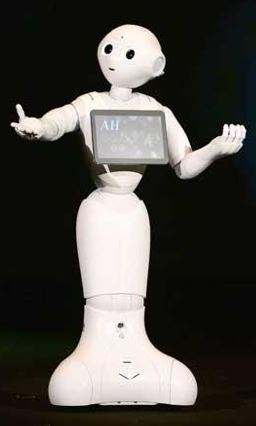
\includegraphics[scale=0.7]{robotPepper}
	\caption{Fotografía del Robot Pepper. \cite{imagen_pepper} }
	\label{fig:RobotPepper}
\end{figure}


Utilizando todas estas herramientas que posee el robot, el problema se puede solucionar de la siguiente manera:

El robot debe estar pendiente de las instrucciones que le indique el paciente, para lo cual, se utilizarán los micrófonos
para grabar el audio (mensaje) emitido por el paciente, posteriormente convertirlo a texto y por último interpretar este
texto como una instrucción. Después de interpretar la instrucción, el robot debe buscar el objeto que le pidió el paciente
mediante el uso de redes neuronales convolucionales de región (en inglés r-cnn: region convolutional neural network).
Si el robot no logra localizarlo, éste deberá notificarle al paciente que no encontró el objeto; por otro lado, si el robot
logra localizar el objeto, éste deberá desplazarse hasta donde está el objeto, sujetar el objeto y llevarlo donde se encuentra
el paciente. El robot debe entregarle el objeto al paciente  en un lugar cercano, por ejemplo, una mesa de noche, con el 
objetivo de velar por la salud y seguridad del paciente. Para términos prácticos el entorno donde se llevará a cabo las 
pruebas y evaluación del proyecto será en el laboratorio de Robótica y Visión Tridimensional en la Universidad de Alicante, España. 
En la figura \ref{fig:DiagramaDeSolucion} se puede brinda un diagrama de flujo que facilita la comprensión de la propuesta para 
hacer frente al problema en cuestión. 



\begin{figure}
	\centering
	\usetikzlibrary{arrows.meta}

\tikzstyle{startstop} = [rectangle, rounded corners, minimum width=3cm, minimum height=1cm,text centered, draw=black, fill=red!30,align=center]

\tikzstyle{io} = [trapezium, trapezium left angle=70, trapezium right angle=110, minimum width=1cm, minimum height=1cm, text centered, draw=black, fill=blue!30,align=center]

\tikzstyle{process} = [rectangle, minimum width=3cm, minimum height=1cm, text centered, draw=black, fill=orange!30,align=center]


\tikzstyle{decision} = [draw, diamond,aspect=2, text centered, draw=black, fill=green!30,inner sep=0pt,align=center]

\tikzstyle{fixedD}=[draw,rectangle split, rectangle split horizontal,align=center,rectangle split parts=3,minimum height=1cm,fill={rgb:red,50;green,200;blue,216}]

\tikzstyle{arrow} = [thick,->,>=stealth]


\newpage
\begin{center}
\begin{tikzpicture}[node distance=1.6cm]

%---------Declaracion de nodos de acción
\node (roslaunch)           [startstop                                                   ] {Inicio Proceso};
\node (espera)              [process , below of=roslaunch                                ] {Estado de espera};
\node (grabar)              [process , below of=espera                                   ] {Grabar audio\\ de instrucción};
\node (traducir)            [process , below of=grabar                                   ] {Traducir audio\\ a texto};
\node (instruccionvalida)   [decision, below of=traducir,node distance=2.3cm             ] {¿Instrucción\\ Valida?};
\node (tomaimagenrgb)       [process , below of=instruccionvalida,node distance=2.3cm    ] {Tomar imagen 2D\\ del entorno};
\node (reconocerobjeto)     [decision, below of=tomaimagenrgb,node distance=2.3cm        ] {¿Objeto\\ Reconocido?};
\node (localizarobjeto)     [process , below of=reconocerobjeto, node distance=2.3cm     ] {Localizar objeto\\ en el entorno};
\node (desplazamiento)      [process , below of=localizarobjeto                          ] {Desplazar el robot hasta el objeto};
\node (tomarobjeto)         [fixedD  , below of=desplazamiento                           ] {\nodepart{two}\shortstack{Tomar objeto\\ con movimientos\\ pregrabados}};
\node (desp_a_paciente)     [process , below of=tomarobjeto                              ] {Desplazar el robot\\ cerca del paciente};
\node (entregarobjeto)      [process , below of=desp_a_paciente                          ] {Entregar el objeto\\ cerca del paciente};
\node (finalizaproceso)     [process , below of=entregarobjeto                           ] {Fin de tarea};


%--------Declaracion de nodos input output
\node (audio)               [io, left of=grabar, xshift=-3cm                             ] {Audio: Mensaje\\ de persona};
\node (imagen2D)            [io, left of=tomaimagenrgb, xshift=-3cm                      ] {Imagen 2D\\ RGB del kinect        };
\node (imagenProfundidad)   [io, left of=localizarobjeto, xshift=-3cm                    ] {Imagen de\\ profundidad\\ del kinect};
\node (inst_no_valida)      [io, right of=instruccionvalida,xshift=4cm                   ] {Respuesta del robot:\\ `Instrucción no valida`};
\node (objeto_no_reconocido)[io, right of=reconocerobjeto,xshift=4cm                     ] {Respuesta del robot:\\ `No se reconoció\\ el objeto`};

%Dibujar flechas de conexion
\draw [arrow] (roslaunch)                  -- (espera);
\draw [arrow] (espera)                     -- (grabar);
\draw [arrow] (grabar)                     -- (traducir);
\draw [arrow] (traducir)                   -- (instruccionvalida);
\draw [arrow] (instruccionvalida)          -- node[anchor=east] {Si}  (tomaimagenrgb);
\draw [arrow] (instruccionvalida)          -- node[anchor=south] {No}  (inst_no_valida);
\draw [arrow] (tomaimagenrgb)              -- (reconocerobjeto);
\draw [arrow] (reconocerobjeto)            -- node[anchor=east] {Si} (localizarobjeto);
\draw [arrow] (reconocerobjeto)            -- node[anchor=south] {No} (objeto_no_reconocido);
\draw [arrow] (localizarobjeto)            -- (desplazamiento); 
\draw [arrow] (desplazamiento)             -- (tomarobjeto);
\draw [arrow] (tomarobjeto)                -- (desp_a_paciente);
\draw [arrow] (desp_a_paciente)            -- (entregarobjeto);
\draw [arrow] (entregarobjeto)             -- (finalizaproceso);
\draw [arrow] (finalizaproceso.west)       -- + (-6,0) |- (espera);
\draw [arrow] (imagen2D)                   -- (tomaimagenrgb);
\draw [arrow] (imagenProfundidad)          -- (localizarobjeto);
\draw [arrow] (audio)                      -- (grabar);
\draw [arrow] (inst_no_valida)             |- (espera);
\draw [arrow] (objeto_no_reconocido.east)  -- + (2,0) |-  (espera);
















\end{tikzpicture}

\end{center}


\newpage
	\caption{Diagrama de Solucion} \label{fig:DiagramaDeSolucion} 
\end{figure}

\newpage



\section{Metodología utilizada en la investigación}
La metodología utilizada en el proceso de investigación debe ser descrita en forma breve o resumida, de tal manera que el lector comprenda cómo se hizo la tesis y qué elementos fueron utilizados para demostrar o negar la hipótesis (diseño de la investigación, tipo de muestreo empleado, tamaño de la muestra, instrumentos empleados para la recopilación de información, etc.).


\newpage




\section{Objetivos de la investigación}

\begin{enumerate}
    \item{\textbf{Objetivo general:}} 
    
    Diseñar un sistema que asista al paciente en la tarea específica de alcanzar objetos 
    según lo requiera la persona utilizando el robot Pepper
    \item{\textbf{Objetivos específicos}}:
    \begin{enumerate}
    \item Implementar el reconocimiento de los objetos específicos en el entorno que rodea al robot.
        \begin{enumerate}
            \item Indicador: El robot debe reconocer tres objetos pequeños mínimo el 90\% de los intentos 
            en un rango de 1 a 5 metros de distancia.
        \end{enumerate}
    
        \item Implementar el reconocimiento de la voz del paciente y traducirlo como una instrucción.
        \begin{enumerate}
            \item Indicador: El robot debe reconocer la siguientes palabras: traer, alcanzar y los tres nombres 
            de los objetos que se deben reconocer, mínimo un 90\% de los intentos cuando esté a 1 metro de 
            distancia o menos del paciente, una vez que el mensaje haya sido traducido de audio a texto.
        \end{enumerate}
        
        \item Integrar las tareas de desplazamiento y el movimiento de objetos por parte del robot junto con 
        el reconocimiento de objetos y de voz. 
        \begin{enumerate}
            \item Entregable: Esta integración debe cumplir con las métricas definidas anteriormente además 
            de solucionar el problema de la siguiente forma: Cuando la instrucción haya sido interpretada, 
            el robot debe buscar el objeto deseado, determinar su ubicación y desplazarse hasta este a una 
            distancia de aproximadamente 35 centímetros, posteriormente deberá tomarlo y llevarlo hasta una 
            posición cerca del paciente de igual manera a una distancia aproximada de 35 centímetros. 
            Si el robot no logra ubicar el objeto, deberá indicarle al paciente que no logró identificarlo.
            
        \end{enumerate}
    \end{enumerate}
\end{enumerate}




\section{Estructura del documento}
Respecto a la explicación breve del contenido de la investigación se debe narrar en qué consiste cada capítulo 
de la tesis de tal manera que el lector decida continuar leyendo toda la tesis o decida ignorarla por no ser un tema de su interés.
